\documentclass[aspectratio=169,10pt]{beamer}
% \usetheme[numbering=fraction,progressbar=frametitle]{metropolis} %
% \usepackage{amsmath, amsfonts, amssymb}
% \usepackage{graphicx}
% \usepackage{booktabs}
% \usepackage{xcolor}
\usepackage{template}
\usepackage{biblatex}
\addbibresource{references.bib}

\title{Federated Learning: a Tale of Heterogeneity}
\author[Paul Mangold]{\textbf{Paul Mangold}}
\institute[CMAP, École Polytechnique]{CMAP, CNRS, École Polytechnique, Institut Polytechnique de Paris}
\date[FLTA 2025]{SIMPAS Group Meeting, November 12, 2025}


% \usepackage{enumitem}

\usepackage{hyperref}
\hypersetup{
    colorlinks=true,
    allcolors=amaranth
  }
  

  
\usepackage{xcolor}
\usepackage{pifont}

\definecolor{amethyst}{rgb}{0.6, 0.4, 0.95}

% Checkmark and cross macros
\newcommand{\cmark}{\textcolor{green!60!black}{\ding{51}}} % ✓
\newcommand{\xmark}{\textcolor{red!70!black}{\ding{55}}}   % ✗

\usepackage{varwidth}
\usepackage{tikz}
\usetikzlibrary{tikzmark}
\setbeamertemplate{itemize items}{\textcolor{amaranth}{\ding{223}}}% \textbullet}}


\tikzset{
    blueblock/.style = {draw=amethyst,fill=amethyst!15,rounded corners=0pt,inner sep=4pt}
}
\tikzset{
    pinkblock/.style = {draw=amaranth,fill=amaranth!15,rounded corners=0pt,inner sep=4pt}
}
\tikzset{
    greyblock/.style = {draw=amaranth,fill=black!5,rounded corners=0pt,inner sep=4pt}
}

\tikzset{
    widepinkblock/.style = {draw=amaranth,fill=amaranth!15,rounded corners=0pt,inner sep=20pt}
}


\begin{document}

%------------------------------------------------
\begin{frame}
  \titlepage
\end{frame}


\begin{frame}{Data Collection}
  \hspace{-3em}
  \begin{minipage}{0.5\linewidth}
    \begin{center}
      Data center\\[0.5em]
      
      \includegraphics[width=0.4\linewidth]{plots/central.pdf}
    \end{center}
    
  \end{minipage}vs.\hspace{1.5em}%
  \begin{minipage}{0.5\linewidth}

    \begin{center}
      Data collection \emph{by users} \\[0.5em]
      
      \includegraphics[width=0.8\linewidth]{plots/decentralized.pdf}
    \end{center}
  \end{minipage}

  \vspace{1em}
  
  \begin{center}
    \textbf{
    $\rightarrow$ how to use all this data?}
  \end{center}
\end{frame}

\begin{frame}{The Traditional Approach to Machine Learning}
  
  \begin{minipage}{0.4\linewidth}
    \begin{center}
      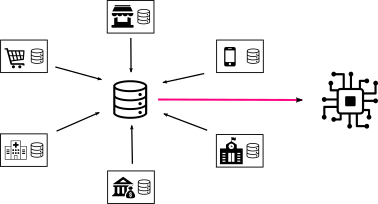
\includegraphics[width=\linewidth]{plots/centralize-data.pdf}
    \end{center}
    
  \end{minipage}~~~~%
  \begin{minipage}{0.5\linewidth}
    \begin{center}
      A single optimization problem      
    \end{center}
    \begin{align*}
      \min_{\theta \in \mathbb{R}^d} \mathbb{E}_{x, y \sim D} \Big[ F( \theta; Z ) \Big]
    \end{align*}
    
  \end{minipage}

\end{frame}

\begin{frame}[t]{Centralizing in a data center is difficult}

  Centralizing data is often impossible
  \begin{itemize}
  \item \emph{Privacy}:

    {\small
    $\rightarrow$ data may be sensitive (e.g. health records, geolocation)
    }
    \\
    ~

  \item \emph{Volume of data}:

    {\small
      $\rightarrow$ data may be large (e.g. high-resolution images, video)
    }
    \\
    ~
    
  \item \emph{Time}:

    {\small
    $\rightarrow$ it may be needed to take decisions quickly (e.g. reinforcement learning)
    }
    
  \end{itemize}

\end{frame}

% \begin{frame}{Why share in the first place?}

%   If it is so difficult to share data... why do it?
%   \begin{itemize}
%   \item local datasets are often too small

%     {\small
%       $\rightarrow$ no statistical significance (e.g. medical study)
%     }
%     \\
%     ~
    
    
%   \item local datasets can be biased

%     {\small
%       $\rightarrow$ if a self-driving car learns in countryside, can it drive in the city?
%     }
%     \\
%     ~
    
        
%   \end{itemize}
  
% \end{frame}




\begin{frame}[t]{Federated Optimization}
% \footfullcite{mangold2020decentralized}$^{,}$\footfullcite{ogier2022flamby}$^{,}$\footfullcite{mangold2024scafflsa}$^{,}$\footfullcite{mangold2025refined}$^{,}$\footfullcite{mangold2025scaffold}}
\vspace{0.5em}
  \begin{minipage}{0.35\linewidth}
    \begin{center}
    \only<1>{    \includegraphics[width=\linewidth]{plots/federated_learning_only_server.pdf} }%
    \only<2,3,4>{    \includegraphics[width=\linewidth]{plots/federated_learning.pdf} }
    \end{center}
    
  \end{minipage}~~~~~~%
  \begin{minipage}{0.5\linewidth}

\only<3,4>{
    \begin{center}
      Collaborative optimization
      \begin{align*}
        \min_{x \in \mathbb{R}^d} 
        \frac{1}{N} \sum_{c=1}^N f_c(x)
        ~~,
        \quad 
        f_c(x)
        = \mathbb{E}_Z[ F_c(x; Z) ]
      \end{align*}
      % $\rightarrow$ with a single \emph{global solution}
    \end{center}
    }
      
  \end{minipage}

\vspace{0.5em}

\only<4>{
  \begin{center}
      \textbf{\textcolor{purple}{Central difficulties}}: data and computational heterogeneity 

      \vspace{-0.5em}
      
      + slow and hard-to-establish communication
  \end{center}
}

\end{frame}


% \begin{frame}{Classical vs Federated Learning}
  
%   \begin{minipage}{0.4\linewidth}
%     \begin{center}
%       \includegraphics[width=\linewidth]{plots/federated-training.pdf}
%     \end{center}
    
%   \end{minipage}~~~~%
%   \begin{minipage}{0.5\linewidth}
%     \begin{center}
%       Multiple sub-problems
%       \begin{align*}
%         \min_{\theta \in \mathbb{R}^d} 
%         \sum_{c=1}^N \mathbb{E}_{x^c, y^c \sim \mathcal{D}^c} \Big[ \ell( \theta; x^c, y^c ) \Big]
%       \end{align*}
      
%       $\rightarrow$ but only \emph{one shared solution}
%     \end{center}
    
%   \end{minipage}


% \end{frame}

\begin{frame}{Best Scenario: Homogeneous Data}

  \begin{minipage}[t]{0.5\linewidth}
    $N$ local sub-problems
    \small
    \begin{align*}
      \min_{\theta \in \mathbb{R}^d}
      \mathbb{E}_{Z \sim \mathcal{D}^1} \Big[ F_1( \theta; Z ) \Big]
      \rightarrow
      \hat\theta_\star^1
    \end{align*}

    \vspace{-2em}
    
    \begin{align*}
      \min_{\theta \in \mathbb{R}^d}
      \mathbb{E}_{Z \sim \mathcal{D}} \Big[ F_2( \theta; Z) \Big]
      \rightarrow
      \hat\theta_\star^2
    \end{align*}

    \vspace{-2em}

    \begin{align*}
      \vdots
    \end{align*}

    \vspace{-2em}
    
    \begin{align*}
      \min_{\theta \in \mathbb{R}^d} 
      \mathbb{E}_{Z \sim \mathcal{D}} \Big[ F_N( \theta; Z ) \Big]
      \rightarrow
      \hat\theta_\star^N
    \end{align*}
  \end{minipage}~~~~%
  \begin{minipage}[t]{0.45\linewidth}
    \pause
    
    Estimate global solution
    \begin{align*}
      \hat\theta_\star
      = \frac{1}{N} \sum_{c=1}^N \hat\theta_\star^c
    \end{align*}

    OK if functions are the same...
  \end{minipage}
  
\end{frame}

\begin{frame}{Best Scenario: Homogeneous Data}
  \vspace{-2em}
  \begin{center}
    \includegraphics[width=0.8\linewidth]{plots/all-minimums-homogeneous.pdf}
  \end{center}
\end{frame}

\begin{frame}{Failure: Heterogeneous Data}
  \vspace{-2em}
  \begin{center}
    \includegraphics[width=0.8\linewidth]{plots/all-minimums-heterogeneous.pdf}
  \end{center}
  \only<2>{%
    \tikz[overlay,remember picture]
    \node[fill=amaranth!10,text=black,inner sep=2em,line width=2pt,draw=amaranth] at ([xshift=0cm,yshift=0cm]current page.center){\LARGE We need a different method...};
  }  
\end{frame}



\begin{frame}{Handling heterogeneity in federated learning}
    % \item \textbf{Federated Learning (FL)}: train models collaboratively without sharing data.
  Challenge: \textcolor{amaranth}{heterogeneity} between clients
  
  \concarrow local drift and bias: clients tend to learn their own solution...
  
  \medskip

  \btca{Two central algorithms in federated learning:}
    
  \begin{itemize}
  \item \textsc{FedAvg}\footfullcite{mcmahan2017communication}: suffers under heterogeneity.

    \concarrow We show it converges in all cases (but is biased!)

  \item \textsc{Scaffold}\footfullcite{karimireddy2020scaffold}: uses \textbf{control variates} to correct drift.
    
  \concarrow We show that it converges in \btca{all regimes!}
  
\end{itemize}
\end{frame}




\begin{frame}[t]{ ~Federated Optimization ~~~ \raisebox{0.2em}{\textcolor{black}{\normalsize $x^\star \in \arg\min_{x \in \mathbb{R}^d} 
    \frac{1}{N} \sum_{c=1}^N \mathbb{E}_Z[ F_c(x; Z) ]$}} ~~}  
    
    \vspace{-1em}

  \begin{minipage}{0.5\linewidth}
  Federated Averaging\footfullcite{mcmahan2017communication} (FedAvg)

\vspace{0.5em}
    

  \footnotesize
  At each global iteration:

    \begin{itemize}
  \footnotesize
    \item For $c=1$ to $N$ in parallel

\vspace{-0.2em}
    
    
\begin{itemize}
\item Receive $x^{(t)}$, initialize $x^{(t,0)}_c = x^{(t)}$
    
        \item For $h=0$ to $H-1$
    \end{itemize}

\vspace{-0.6em}
\begin{center}
            \hspace{-1em}$x^{(t,h+1)}_c = x^{(t,h)}_c - \gamma \nabla F_c( x^{(t,h)}_c ; Z_c^{(t,h+1)})$
        \end{center}
      
  \item Model aggregation
        
        
\vspace{-0.6em}
\begin{center}
            \hspace{-1em}$x^{(t+1)} = \frac{1}{N} \sum_{c=1}^N x_c^{(t,H)}$
        \end{center}
      
    \end{itemize}
      
  \end{minipage}~%
  \begin{minipage}{0.48\linewidth}
  \pause
       \begin{center}
    \includegraphics[width=0.75\linewidth]{plots/local_training_heterogeneous.pdf}%
    \raisebox{2.5em}{ \includegraphics[width=0.25\linewidth]{plots/legend.pdf} }
  \end{center}
  
    \vspace{-0.5em}

  ~~~~More local iterations

    \vspace{0.5em}
    
    ~~~~~{\large \cmark}\, faster convergence
    
    ~~~~~{\large \xmark}~ larger bias

  \end{minipage}

  \vspace{1.5em}


\end{frame}

\begin{frame}[t]{Focus: Analysis of Stochastic FedAvg\footfullcite{mangold2025refined}}

What can we say about the convergence of FedAvg? In the stochastic setting?
  \vspace{-1em} 
  \pause

  \begin{center}
    
  \resizebox{0.9\linewidth}{!}{
  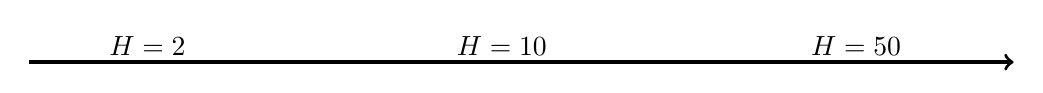
\begin{tikzpicture}
    \draw [-to,very thick](0,0) -- (12.5,0);
    \node at (1.5,0.2) {$H=2$};
    \node at (6,0.2) {$H=10$};
    \node at (10.5,0.2) {$H=50$};
  \end{tikzpicture}
}
\vspace{-0.5em}

  \includegraphics[width=0.3\linewidth]{plots/fedavg_True_2_t1000_s1.pdf}
  \includegraphics[width=0.3\linewidth]{plots/fedavg_True_10_t1000_s1.pdf}
  \includegraphics[width=0.3\linewidth]{plots/fedavg_True_50_t1000_s1.pdf}

\vspace{-3em}

\includegraphics[width=0.8\linewidth]{plots/legend_fedavg.pdf}    
    
  \end{center}

  \vspace{-3em}

  \pause
  \begin{tikzpicture}[remember picture, overlay]
        \node[widepinkblock]
        at (current page.center) {
        \huge
        Short answer: the algorithm converges!
        };
    \end{tikzpicture}
\end{frame}


\begin{frame}[t]{Focus: Analysis of Stochastic FedAvg\footfullcite{mangold2025refined}}

{\small If each $f_c$ is three times differentiable, $\mu$-strongly convex, $\nabla f_c$ is $L$-Lipschitz, and $\gamma \le 1/L$}
\begin{itemize}
    \item FedAvg converges in Wasserstein distance to a distribution $\pi^{(\gamma, H)}$
    \only<2>{
    \begin{itemize}
        \item and if $x^{(t)} \sim \psi_{x^{(t)}}$,
    \begin{align*}
        \mathcal{W}_2(\psi_{x^{(t)}}; \pi^{(\gamma, H)})
        \le
        (1 - \gamma \mu)^{H t} \mathcal{W}_2(\psi_{x^{(0)}}; \pi^{(\gamma, H)})
    \end{align*}
    \item where $\mathcal{W}_2$ is the 2-Wasserstein distance
    \end{itemize}
    }

\pause

\pause


    \item Bias of FedAvg (for small $\gamma, H$) 
    \only<3,4,5>{
    \begin{align*}
    \int x \pi^{(\gamma, H)}(\mathrm{d} x)
    &  = x^\star +
    \tikz[remember picture,baseline=(heterbias.base)] \node[blueblock] (heterbias) at (0,0) {
    \textnormal{$\displaystyle \frac{\gamma (H-1)}{2N}
    \sum_{c=1}^N \nabla^2 f(x^\star)^{-1}
    \big( \nabla^2 f_c(x^\star) - \nabla^2 f(x^\star) \big)
    \nabla f_c(x^\star)$}
    };
    \\ 
    &  \qquad
    -  \tikz[remember picture,baseline=(stobias.base)] \node[pinkblock] (stobias) at (0,0) {
    \textnormal{$\displaystyle
    \frac{\gamma}{2 N} \nabla^2 f(x^\star)^{-1}
    \nabla^3 f(x^\star) A^{-1} C(x^\star)
    $}};
    + O(\gamma^2 H^2)
    \end{align*}
    }
\pause

\only<3,4,5>{
\begin{tikzpicture}[overlay,remember picture]
    \node[blueblock] (heterbiaslegend) at (3,5) {\shortstack{\underline{Heterogeneity bias} \\[0.5em]
     Disappears when $\nabla^2 f_c(x^\star) = \nabla^2 f(x^\star)$ \\
    \quad or when $\nabla f_c(x^\star) = \nabla f(x^\star)$
    }};
    \draw[color=amethyst] (heterbias) -- (heterbiaslegend);
    
    \node[pinkblock] (stobiaslegend) at (10,5) {\shortstack{\underline{Stochasticity bias} \\[0.5em]
    $A$ is a linear operator \\
    $C(x^\star)$ is the covariance of $\nabla f$ at $x^\star$
    }};
    \draw[color=amaranth] (stobias) -- (stobiaslegend);
\end{tikzpicture}

\vspace{-4em}
}

% \pause
% \item Richardson-Romberg extrapolation
% \begin{itemize}
%     \item Combine FedAvg with steps $\gamma$ and $2 \gamma$ to \textbf{reduce bias}
%     %\item \textbf{No additional memory cost!}
% \end{itemize}


\end{itemize}

\only<5>{
\begin{tikzpicture}[remember picture, overlay]
        \node[widepinkblock,line width=2pt]
        at (current page.center) {
        \huge How to fix this heterogeneity bias?};
    \end{tikzpicture}
}




\end{frame}

%------------------------------------------------

\begin{frame}{Mitigating Heterogeneity: Scaffold}

\begin{itemize}
  \item A classical algorithm to mitigate heterogeneity in federated learning is \textbf{\textsc{Scaffold}} \footfullcite{karimireddy2020scaffold}.
  \item First it performs local updates
  \[
    \theta_{t,h+1}^c = \theta_{t,h}^c - \gamma \big(\nabla f_c(\theta_{t,h}^c) - \xi_t^c\big),
  \]
  \item Then local updates are aggregated, and control variates updated
    \begin{align*}
      \theta_{t+1} & = \frac{1}{N}\sum_{c=1}^N \theta_{t,H}^c \\
      \xi_{t+1}^c & = \xi_t^c + \frac{1}{\gamma H}(\theta_{t,H}^c - \theta_{t+1})
  \end{align*}
\item \textsc{Scaffold} {accelerates training} by reducing client drift caused by data heterogeneity but:
  \begin{itemize}
  \item does it converge in any setting like FedAvg?
  \item does it actually correct heterogeneity?
  \item what is the correct rate?
  \end{itemize}
  \vspace{1em}
\end{itemize}

\end{frame}


\begin{frame}{Let's study the quadratic case!}
We minimize the quadratic FL objective:
\[
\min_{\theta\in\mathbb{R}^d} \frac{1}{N} \sum_{c=1}^N \Big( \tfrac{1}{2}\theta^\top A_c\theta - b_c^\top\theta \Big),
\]
with $A_c \succ 0$ with eigenvalues between $\mu$ and $L$, heterogeneous across clients.
\pause

\textbf{\textsc{Scaffold} updates (deterministic, but our results also cover stochastic case):}
\[
\theta_{t,h+1}^c = \theta_{t,h}^c - \gamma (A_c \theta_{t,h}^c - b_c + \xi_t^c)
\]
\[
  \theta_{t+1} = \frac{1}{N} \sum_{c=1}^N \theta_{t,H}^c
  \qquad
  \xi_{t+1}^c = \xi_t^c + \frac{1}{\gamma H} (\theta_{t,H}^c - \theta_{t+1})
\]
\vspace{0.4em}
\begin{itemize}
  \item Control variates $\xi_c$ estimate gradient at optimum.
  \item Bias correction mitigates client drift.
\end{itemize}
\end{frame}



%------------------------------------------------
\begin{frame}{What are the properties of Scaffold?}
\textcolor{amaranth}{Goal:} 
Provide a \textbf{refined theoretical analysis} of \textsc{Scaffold} for quadratic objectives.

\begin{block}{\normalsize Contributions:}
\begin{itemize}
  \item We establish convergence for \emph{any number of local steps}

    ...by decomposing dynamics along the \textbf{eigenspaces of the Hessian}.
    
  \item We identify optimal scaling of the number of local updates:
  \[
  H_\gamma \propto \frac{1}{\gamma\sqrt{\mu L}}.
  \]
  \end{itemize}
\end{block}

\vspace{-2.5em}

\begin{center}
  \foreach \h in {1, 10, 100, 1000} {
    \includegraphics[width=0.23\linewidth]{plots/quadratic_scaffold_h\h_t100_s1.pdf}%
  }
  Blue: FedAvg, \quad Pink: Scaffold. Left to right: $1, 10, 100, 1000$ local steps
\end{center}

\end{frame}

%------------------------------------------------

%------------------------------------------------
\begin{frame}{Spectral Decomposition of the Updates}

\textcolor{amaranth}{Main Result:} assume $\mu I \preccurlyeq A_c \preccurlyeq L I$, and $\gamma \le 1/L$. For any number of local steps $H > 0$,
\[
\mathbb{E}[\|X_{t+1} - X_{*}\|_\Lambda^2] 
\le \rho_{\gamma,H} \, \mathbb{E}[\|X_t - X_* \|_\Lambda^2],
\]
where $X_t = (\theta_t, \xi_t^1, \dots, \xi_t^N)$ and $X_* = (\theta_*, \xi_*^1, \dots, \xi_*^N)$
\[
\rho_{\gamma,H} = \max\!\left\{ (1-\gamma\mu)^H, \, 1 - \frac{1 - 1/e}{\gamma L H} \right\} < 1.
\]

\textcolor{amaranth}{Proof idea:}
\begin{itemize}
  \item Write each local Hessian: $A_c = U_c D_c U_c^\top$.
  \item Decompose the dynamics along eigen-directions of $A_c$.
  \item This per-eigenvalue analysis of contraction!
  \end{itemize}


  \begin{center}
    \concarrow \btca{\large \textsc{Scaffold} remains convergent for all $H$!}
  \end{center}
      


\end{frame}

%------------------------------------------------
\begin{frame}{Interpretation of the Contraction Rate}
  For each eigenvalue $a$ of $A_c$:
  \begin{itemize}
  \item Two regimes:
    \begin{itemize}
    \item $\gamma a H \le 1$: exponential decay $(1 - \gamma a)^H \le (1 - \gamma \mu)^H$
      \btca{$\rightarrow$ faster with larger $H$}
    \item $\gamma a H > 1$: algebraic decay $1 - \tfrac{1 - 1/e}{\gamma a H} \le 1 - \tfrac{1 - 1/e}{\gamma L H}$
      \btca{$\rightarrow$ slower with larger $H$}
    \end{itemize}
  \item Transition when $\gamma a H = 1$.
  \end{itemize}
  
  \centering
  \includegraphics[width=0.5\linewidth]{plots/contract_rate_max_term.pdf}%
  \raisebox{2em}{\includegraphics[width=0.16\linewidth]{plots/contract_rate_max_term_legend.pdf}}
  \\[0.3em]
  \scriptsize{Contraction rate vs number of local steps.}
\end{frame}

%------------------------------------------------
\begin{frame}{Acceleration and Optimal Local Steps}
Balancing the two regimes requires setting:
\[
(1-\gamma\mu)^H = 1 - \frac{1 - 1/e}{\gamma L H}
\Rightarrow \tca{\boldsymbol{H_\gamma = \left\lceil \sqrt{ \frac{2(1-1/e)}{\gamma^2 L \mu} } \right\rceil}}
\]
\pause
\begin{itemize}
\item Optimal rate:
  \vspace{-2em}
  \[
  \rho_{\text{opt}} = 1 - \sqrt{ \frac{2(1 - 1/e)\mu}{L} }.
\]

\vspace{2em}

  \item Communication complexity:
  \vspace{-2em}
  \[
  T = O\!\left( \sqrt{\frac{L}{\mu}} \log \frac{1}{\varepsilon} \right),
  \]
  i.e., $\sqrt{L/\mu}$ improvement over FedAvg.
\end{itemize}

Recovers both the rates of ProxSkip and its refined analyses... but without stochastic communication scheme.\footfullcite{mishchenko2022proxskip}$^{,}$\footfullcite{hu2023tighter}

\vspace{1em}
\end{frame}

%------------------------------------------------
\begin{frame}{Extension to Stochastic Setting}
  \textsc{Scaffold} with noise converges to a unique stationary distribution.
  Its variance $\Sigma_X$ satisfies:
  \[
  \Sigma_X = A_{\gamma,H}\Sigma_X A_{\gamma,H}^\top + B_{\gamma,H}.
  \]
\pause
\tca{Result on variance:} for homogeneous quadratics, $\text{tr}(\Sigma_\theta) \lesssim \frac{\gamma\sigma^2}{N}$

\concarrow Linear speed-up with number of clients $N$.

\btca{Conjectures:}
\begin{itemize}
\item this result still holds in heterogeneous settings
\item this result still holds in non-linear (strongly-convex) case
\end{itemize}
\end{frame}

%------------------------------------------------
\begin{frame}{Numerical Results}
\begin{columns}
\column{0.60\textwidth}
\begin{itemize}
  \item \textsc{Scaffold} converges for all $H$ if $\gamma \le 1/L$.
  \item Accelerated convergence up to optimal $H_\gamma$.
  \item Variance decreases linearly with number of clients.
\end{itemize}
\column{0.4\textwidth}
\centering
$N=10$, $\gamma=1$:
\includegraphics[width=0.8\linewidth]{plots/convergence_step1_h2000_sigma0.01.pdf}
\\[0.3em]
$H=10$, $\gamma=1$:
\includegraphics[width=0.8\linewidth]{plots/convergence_step1_nclients_sigma0.1.pdf}
\\[0.3em]
% \scriptsize{Mean-squared error vs communications.}
\end{columns}
\end{frame}

%------------------------------------------------
\begin{frame}{Discussion and Perspectives}
  We have developed a framework for studying federated algorithms
  \begin{itemize}
  \item study the \btca{convergence} of the algorithm to its limit
  \item determine how far the algorithm's limit is from the solution
  \end{itemize}
  This gives novel analyses of FedAvg and Scaffold!

  There are still many open problems to solve!!
  
  \concarrow \btca{Lucas' talk:} what about \btca{decentralized} optimization?

  
\end{frame}

\begin{frame}{Beyond the classical FL: Federated Reinforcement Learning}

  Idea: make RL agents collaborate to solve these problems together \textbf{faster}

  \vspace{-1em}
  \begin{center}
  \resizebox{!}{14em}{
      \begin{tikzpicture}[scale=0.8,->,>=stealth',auto,node distance=3cm,
        thick,main node/.style={circle,draw,font=\sffamily\Large\bfseries}]
        % nodes 
        \node[draw,fill=white, align=center, inner sep=5pt] (A1) at (0, 1.5) {agent 1 \\ $s_t^{(1)}$};
        \node[draw, fill=white, align=center, inner sep=5pt] (B1) at (0, 0) {env 1};

        
        \node[draw,fill=white, align=center, inner sep=5pt] (A2) at (0, -1.5) {agent 2 \\ $s_t^{(2)}$};
        \node[draw, fill=white, align=center, inner sep=5pt] (B2) at (0, -3) {env 2};

        \node (dots) at (0, -4) {$\cdots$};
        
        \node[draw,fill=white, align=center, inner sep=5pt] (An) at (0, -5.5) {agent n \\ $s_t^{(n)}$};
        \node[draw, fill=white, align=center, inner sep=5pt] (Bn) at (0, -7) {env n};


        % arrows
        \draw [->] (B1.west) to [out=180,in=180] (A1.west) ;
        \draw [->] (A1.east) to [out=0,in=0] (B1.east);
        \draw [->] (B2.west) to [out=180,in=180] (A2.west) ;
        \draw [->] (A2.east) to [out=0,in=0] (B2.east);
        \draw [->] (Bn.west) to [out=180,in=180] (An.west) ;
        \draw [->] (An.east) to [out=0,in=0] (Bn.east);

        \node[align=center,inner sep=15pt] (A1t) at (-1.7, 0.75) {$r_t^{(1)}$ \\[0.5em] $S_{t+1}^{(1)}$};
        \node[align=center,inner sep=15pt] (B1t) at (1.8, 0.75) {$a_t^{(1)}$};
        \node[align=center,inner sep=15pt] (C1t) at (-4, 0.75) {\includegraphics[width=4em]{plots/sedan-car-icon.pdf}};

        \node[align=center,inner sep=15pt] (A2t) at (-1.7, -2.25) {$r_t^{(2)}$ \\[0.5em] $S_{t+1}^{(2)}$};
        \node[align=center,inner sep=15pt] (B2t) at (1.8, -2.25) {$a_t^{(2)}$};

        \node[align=center,inner sep=15pt] (C2t) at (-4, -2.25) {\includegraphics[width=4em]{plots/logistic-van-icon.pdf}};


        \node[align=center,inner sep=15pt] (Ant) at (-1.7, -6.25) {$r_t^{(n)}$ \\[0.5em] $S_{t+1}^{(n)}$};
        \node[align=center,inner sep=15pt] (Bnt) at (1.8, -6.25) {$a_t^{(n)}$};

        \node[align=center,inner sep=15pt] (Cnt) at (-4, -6.25)  {\includegraphics[width=4em]{plots/suv-car-icon.pdf}};

        \node[fill=white, align=center, inner sep=5pt] (model) at (12, -2.7) {global policy};

        \node[draw, fill=white, align=center, inner sep=24pt] (algo) at (7, -2.7) {central server};
        % arrows
        \draw[<->] (B1t) to (algo);
        \draw[<->] (B2t) to (algo);
        \draw[<->] (Bnt) to (algo);
        \draw[->] (algo) to (model);

      \end{tikzpicture}   

    }
    
  \end{center}
  \vspace{-1em}
  \vspace{-1em}
  Methods of reinforcement learning differ a lot from classical optimization: what about federated?

  % See the talks of
  % \begin{itemize}
  % \item \btca{Safwan:} federated value iteration with heterogeneity
  % \item \btca{Lorenzo:} towards personalization in federated reinforcement learning
  % \end{itemize}
\end{frame}

%------------------------------------------------
\begin{frame}{Questions?}

  Next talks for this SGM:
  \begin{itemize}
  \item \btca{Lucas:} \textit{Analysis of Decentralized SGD: a Markov Chain Perspective}

    $\rightarrow$ what if we don't have a central server?
    
  \item \btca{Safwan:} \textit{Federated Model-Based Reinforcement Learning}

    $\rightarrow$ how to estimate collaboratively the environments of each agents?
    
  \item \btca{Lorenzo:} \textit{Personalized Federated Reinforcement Learning}

    $\rightarrow$ beyond global model: how can we personalize the models?
  \end{itemize}
\end{frame}

\end{document}

%%% Local Variables:
%%% mode: LaTeX
%%% TeX-master: t
%%% End:
